% Options for packages loaded elsewhere
\PassOptionsToPackage{unicode}{hyperref}
\PassOptionsToPackage{hyphens}{url}
%
\documentclass[
  ignorenonframetext,
  serif,
  professionalfont,
  usenames,
  dvipsnames,
  aspectratio = 169]{beamer}
\usepackage{pgfpages}
\setbeamertemplate{caption}[numbered]
\setbeamertemplate{caption label separator}{: }
\setbeamercolor{caption name}{fg=normal text.fg}
\beamertemplatenavigationsymbolsempty
% Prevent slide breaks in the middle of a paragraph
\widowpenalties 1 10000
\raggedbottom
\setbeamertemplate{part page}{
  \centering
  \begin{beamercolorbox}[sep=16pt,center]{part title}
    \usebeamerfont{part title}\insertpart\par
  \end{beamercolorbox}
}
\setbeamertemplate{section page}{
  \centering
  \begin{beamercolorbox}[sep=12pt,center]{part title}
    \usebeamerfont{section title}\insertsection\par
  \end{beamercolorbox}
}
\setbeamertemplate{subsection page}{
  \centering
  \begin{beamercolorbox}[sep=8pt,center]{part title}
    \usebeamerfont{subsection title}\insertsubsection\par
  \end{beamercolorbox}
}
\AtBeginPart{
  \frame{\partpage}
}
\AtBeginSection{
  \ifbibliography
  \else
    \frame{\sectionpage}
  \fi
}
\AtBeginSubsection{
  \frame{\subsectionpage}
}
\usepackage{amsmath,amssymb}
\usepackage{lmodern}
\usepackage{iftex}
\ifPDFTeX
  \usepackage[T1]{fontenc}
  \usepackage[utf8]{inputenc}
  \usepackage{textcomp} % provide euro and other symbols
\else % if luatex or xetex
  \usepackage{unicode-math}
  \defaultfontfeatures{Scale=MatchLowercase}
  \defaultfontfeatures[\rmfamily]{Ligatures=TeX,Scale=1}
\fi
% Use upquote if available, for straight quotes in verbatim environments
\IfFileExists{upquote.sty}{\usepackage{upquote}}{}
\IfFileExists{microtype.sty}{% use microtype if available
  \usepackage[]{microtype}
  \UseMicrotypeSet[protrusion]{basicmath} % disable protrusion for tt fonts
}{}
\makeatletter
\@ifundefined{KOMAClassName}{% if non-KOMA class
  \IfFileExists{parskip.sty}{%
    \usepackage{parskip}
  }{% else
    \setlength{\parindent}{0pt}
    \setlength{\parskip}{6pt plus 2pt minus 1pt}}
}{% if KOMA class
  \KOMAoptions{parskip=half}}
\makeatother
\usepackage{xcolor}
\newif\ifbibliography
\usepackage{graphicx}
\makeatletter
\def\maxwidth{\ifdim\Gin@nat@width>\linewidth\linewidth\else\Gin@nat@width\fi}
\def\maxheight{\ifdim\Gin@nat@height>\textheight\textheight\else\Gin@nat@height\fi}
\makeatother
% Scale images if necessary, so that they will not overflow the page
% margins by default, and it is still possible to overwrite the defaults
% using explicit options in \includegraphics[width, height, ...]{}
\setkeys{Gin}{width=\maxwidth,height=\maxheight,keepaspectratio}
% Set default figure placement to htbp
\makeatletter
\def\fps@figure{htbp}
\makeatother
\setlength{\emergencystretch}{3em} % prevent overfull lines
\providecommand{\tightlist}{%
  \setlength{\itemsep}{0pt}\setlength{\parskip}{0pt}}
\setcounter{secnumdepth}{-\maxdimen} % remove section numbering
% Definição do esquema de cores:
% 1. UFPR - Azul com cinza.
% 2. DEST - Roxo com cinza.
% 3. LEG - Laranjado com cinza.
\def\mycolorscheme{1}

% Caminho para a imagem de fundo com aspecto 16x9.
% \def\pathtobg{config/ufpr-fachada-baixo-1.jpg}
% \def\pathtobg{config/ufpr-fundo.jpg}
% \def\pathtobg{config/ufpr-fundo.jpg}
\def\pathtobg{./config/ufpr-fundo-16x9.jpg}

% \providecommand{\tightlist}{%
%   \setlength{\itemsep}{0pt}\setlength{\parskip}{0pt}}
% ATTENTION: Redefine o comando acima que é definido pelo template.
% \renewcommand{\tightlist}{}
\renewcommand{\tightlist}{%
  \setlength{\itemsep}{0\baselineskip}
  \setlength{\parskip}{0.25\baselineskip}
}

% Logo na capa.
\titlegraphic{
  %\vspace{-1em}
  %\includegraphics[height=1.2cm]{config/dest-texto-2.png}\hspace{1em}
  %\includegraphics[height=1.8cm]{config/dsbd-logo-2x2.png}\hspace{1em}
  
\includegraphics[height=1.8cm]{config/ufpr-transparent-600px.png}
}
%-----------------------------------------------------------------------

% Palladio.
% \usepackage[sc]{mathpazo}
% \linespread{1.05}         % Palladio needs more leading (space between lines)
% \usepackage[T1]{fontenc}

% Kurier.
% \usepackage[light, condensed, math]{kurier}
% \usepackage[T1]{fontenc}

% Iwona.
% \usepackage[math, light, condensed]{iwona}

% \usepackage{cmbright}
% \usepackage[charter]{mathdesign}
% \usepackage{palatino}

% Roboto (with Iwona for maths).
% \usepackage[math]{iwona}
% \usepackage[sfdefault, light, condensed]{roboto}

% Source Sans Pro (with Iwona for maths).
% \usepackage[math]{iwona}
% \usepackage[default, light]{sourcesanspro}

% Lato (with Iwona for maths).
% \usepackage[math]{iwona}
% \usepackage[default]{lato}

% Fira Sans (with Iwona for maths).
\usepackage[math, light]{iwona}
\usepackage[sfdefault,light]{FiraSans} %% option 'sfdefault' activates Fira Sans as the default text font
\usepackage[T1]{fontenc}
\renewcommand*\oldstylenums[1]{{\firaoldstyle #1}}

% Font for code. ----------------------------
% \usepackage[scaled=.75]{beramono}
\usepackage{inconsolata}

% ATTENTION: needs complile with xelatex: `$ xelatex file.tex`
% \usepackage{fontspec}
% \setmonofont{M+ 1m}
% \setmonofont{M+ 1mn}
% \setmonofont{M+ 2m}

%-----------------------------------------------------------------------

% \usepackage{lmodern}
\usepackage{amssymb, amsmath}
\usepackage[makeroom]{cancel}
% \usepackage{ifxetex, ifluatex}
\usepackage{fixltx2e} % provides \textsubscript
\usepackage[utf8]{inputenc}
\usepackage[shorthands=off,main=brazil]{babel}
\usepackage{graphicx}
\usepackage{xcolor}
\usepackage{setspace}
\usepackage{comment}
\usepackage{icomma}

%-----------------------------------------------------------------------
% Algumas configurações.

\setlength{\parindent}{0pt}
\setlength{\parskip}{6pt plus 2pt minus 1pt}
\setlength{\emergencystretch}{3em}  % prevent overfull lines
% \providecommand{\tightlist}{%
%   \setlength{\itemsep}{0pt}\setlength{\parskip}{0pt}}
\setcounter{secnumdepth}{0}

% Espaço vertical para o ambiente `quote`.
\let\oldquote\quote
\let\oldendquote\endquote
\renewenvironment{quote}{%
  \vspace{1em}\oldquote}{%
  \oldendquote\vspace{1em}}

%-----------------------------------------------------------------------
% Espaçamento entre items para itemize, enumerate e description.

% % itemize.
% \let\itemopen\itemize
% \let\itemclose\enditemize
% \renewenvironment{itemize}{%
%   \itemopen\addtolength{\itemsep}{0.25\baselineskip}}{\itemclose}
%
% % enumerate.
% \let\enumopen\enumerate
% \let\enumclose\endenumerate
% \renewenvironment{enumerate}{%
%   \enumopen\addtolength{\itemsep}{0.25\baselineskip}}{\enumclose}
%
% % description.
% \let\descopen\description
% \let\descclose\enddescription
% \renewenvironment{description}{%
%   \descopen\addtolength{\itemsep}{0.25\baselineskip}}{\descclose}

%-----------------------------------------------------------------------

% \usepackage[hang]{caption}
\usepackage{caption}
\captionsetup{font=footnotesize,
  labelfont={color=mycolor1, footnotesize},
  labelsep=period}

% \providecommand{\tightlist}{%
%   \setlength{\itemsep}{0pt}\setlength{\parskip}{0pt}}

%-----------------------------------------------------------------------

\usepackage{tikz}

% \def\pathtobg{/home/walmes/Projects/templates/COMMON/ufpr-fundo.jpg}
% \def\pathtobg{/home/walmes/Projects/templates/COMMON/ufpr-fundo-16x9.jpg}
% \def\pathtobg{/home/walmes/Projects/templates/COMMON/ufpr-fachada-dir-1.jpg}
% \def\pathtobg{/home/walmes/Projects/templates/COMMON/ufpr-fachada-esq-1.jpg}
% \def\pathtobg{/home/walmes/Projects/templates/COMMON/ufpr-perto-1.jpg}
% \def\pathtobg{/home/walmes/Projects/templates/COMMON/ufpr-fachada-baixo-1.jpg}

\ifx\pathtobg\undefined
\else
  \usebackgroundtemplate{
    \tikz[overlay, remember picture]
    \node[% opacity=0.3,
          at=(current page.south east),
          anchor=south east,
          inner sep=0pt] {
            \includegraphics[height=\paperheight, width=\paperwidth]{\pathtobg}};
  }
\fi

%-----------------------------------------------------------------------
% Definições de esquema de cores.

\ifx\mycolorscheme\undefined
  % UFPR.
  % http://www.color-hex.com/color-palette/2018
  \definecolor{mycolor1}{HTML}{015c93} % Título.
  \definecolor{mycolor2}{HTML}{363435} % Texto.
  \definecolor{mycolor3}{HTML}{015c93} % Estrutura.
  \definecolor{mycolor4}{HTML}{015c93} % Links.
  \definecolor{mycolor5}{HTML}{CECAC5} % Preenchimentos.
\else
  \if\mycolorscheme1
    % UFPR.
    \definecolor{mycolor1}{HTML}{015c93} % Título.
    \definecolor{mycolor2}{HTML}{363435} % Texto.
    \definecolor{mycolor3}{HTML}{015c93} % Estrutura.
    \definecolor{mycolor4}{HTML}{015c93} % Links.
    \definecolor{mycolor5}{HTML}{CECAC5} % Preenchimentos.
  \fi
  \if\mycolorscheme2
    % DEST.
    \definecolor{mycolor1}{HTML}{2a0e72} % Título.
    \definecolor{mycolor2}{HTML}{202E35} % Texto.
    \definecolor{mycolor3}{HTML}{2a0e72} % Estrutura.
    % \definecolor{mycolor3}{HTML}{8072a3} % Estrutura.
    \definecolor{mycolor4}{HTML}{2a0e72} % Links.
    % \definecolor{mycolor4}{HTML}{bfb9d1} % Links.
    % \definecolor{mycolor5}{HTML}{AEA79F} % Preenchimentos.
    \definecolor{mycolor5}{HTML}{CECAC5} % Preenchimentos.
  \fi
  \if\mycolorscheme3
    % LEG.
    \definecolor{mycolor2}{HTML}{363435} % Texto.
    % \definecolor{mycolor1}{HTML}{ff8000} % Título.
    % \definecolor{mycolor3}{HTML}{ff8000} % Estrutura.
    % \definecolor{mycolor4}{HTML}{ff8000} % Links.
    % \definecolor{mycolor1}{HTML}{E57300} % Título.
    % \definecolor{mycolor3}{HTML}{E57300} % Estrutura.
    % \definecolor{mycolor4}{HTML}{E57300} % Links.
    \definecolor{mycolor1}{HTML}{F67014} % Título.
    \definecolor{mycolor3}{HTML}{F67014} % Estrutura.
    \definecolor{mycolor4}{HTML}{F67014} % Links.
    % \definecolor{mycolor1}{HTML}{FE5C23} % Título.
    % \definecolor{mycolor3}{HTML}{FE5C23} % Estrutura.
    % \definecolor{mycolor4}{HTML}{FE5C23} % Links.
    \definecolor{mycolor5}{HTML}{222222} % Preenchimentos.
    \definecolor{mycolor5}{HTML}{383838} % Preenchimentos.
  \fi
\fi

\hypersetup{
  colorlinks=true,
  linkcolor=mycolor4,
  urlcolor=mycolor1,
  citecolor=mycolor1
}

%-----------------------------------------------------------------------
% ATTENTION: http://www.cpt.univ-mrs.fr/~masson/latex/Beamer-appearance-cheat-sheet.pdf

\usetheme{Boadilla}
\usecolortheme{default}

% \setbeamersize{text margin left=7mm, text margin right=7mm}
% \setbeamertemplate{frametitle}[default][left, leftskip=3mm]
% \addtobeamertemplate{frametitle}{\vspace{0.5em}}{}

\setbeamertemplate{caption}[numbered]
\setbeamertemplate{section in toc}[sections numbered]
\setbeamertemplate{subsection in toc}[subsections numbered]
\setbeamertemplate{sections/subsections in toc}[ball]{}
\setbeamertemplate{sections in toc}[ball]
\setbeamercolor{section number projected}{bg=mycolor1, fg=white}
\setbeamertemplate{blocks}[rounded]
\setbeamertemplate{navigation symbols}{}
\setbeamertemplate{frametitle continuation}{\gdef\beamer@frametitle{}}
% \setbeamertemplate{frametitle}[default][center]
% \setbeamertemplate{footline}[frame number]

\setbeamertemplate{enumerate items}[default]
\setbeamertemplate{itemize items}{\scriptsize\raise1.25pt\hbox{\donotcoloroutermaths$\blacktriangleright$}}

% Blocos.
% \addtobeamertemplate{block begin}{\vskip -\bigskipamount}{}
% \addtobeamertemplate{block end}{}{\vskip -\bigskipamount}
\addtobeamertemplate{block begin}{\vspace{0.5em}}{}
\addtobeamertemplate{block end}{}{\vspace{0.5em}}


% Rodapé.
\setbeamercolor{title in head/foot}{parent=subsection in head/foot}
\setbeamercolor{author in head/foot}{bg=mycolor4, fg=white}
\setbeamercolor{date in head/foot}{parent=subsection in head/foot, fg=mycolor3}

% Cabeçalho.
\setbeamercolor{section in head/foot}{bg=mycolor2, fg=mycolor4}
\setbeamercolor{subsection in head/foot}{bg=mycolor2, fg=white}

\setbeamercolor{title}{fg=mycolor1}       % Título dos slides.
\setbeamercolor{titlelike}{fg=title}
\setbeamercolor{subtitle}{fg=mycolor2}    % Subtítulo.
\setbeamercolor{institute in head/foot}{parent=palette primary} % Instituição.
\setbeamercolor{frametitle}{fg=mycolor1}  % De quadro.
\setbeamercolor{structure}{fg=mycolor3}   % Listas e rodapé.
\setbeamercolor{item projected}{bg=mycolor2}
\setbeamercolor{block title}{bg=mycolor5, fg=mycolor2}
\setbeamercolor{normal text}{fg=mycolor2} % Texto.
\setbeamercolor{caption name}{fg=normal text.fg}
% \setbeamercolor{footlinecolor}{fg=mycolor2, bg=mycolor5}
% \setbeamercolor{section in head/foot}{fg=mycolor2, bg=mycolor5}
\setbeamercolor{author in head/foot}{fg=white, bg=mycolor1}
\setbeamercolor{section in foot}{fg=mycolor4, bg=mycolor5}
\setbeamercolor{date in foot}{fg=mycolor4, bg=mycolor5}
\setbeamercolor{block title}{fg=white, bg=mycolor1}
\setbeamercolor{block body}{fg=black, bg=white!80!gray}
\setbeamercolor{block body}{fg=black, bg=white!80!gray}

% To remove empty brackets of \institution.
\makeatletter
\setbeamertemplate{footline}{
  \leavevmode%
  \hbox{%
    \begin{beamercolorbox}[
      wd=0.3\paperwidth, ht=2.25ex, dp=1ex, right]{author in head/foot}%
      \usebeamerfont{author in head/foot}\insertshortauthor{}\hspace*{1ex}
    \end{beamercolorbox}%
    \begin{beamercolorbox}[
      wd=0.6\paperwidth, ht=2.25ex, dp=1ex, left]{section in foot}%
      \usebeamerfont{title in head/foot}\hspace*{1ex}\insertshorttitle{}
      % \usebeamerfont{title in head/foot}\hspace*{1ex}\insertframetitle{}
    \end{beamercolorbox}%
    \begin{beamercolorbox}[
      wd=0.1\paperwidth, ht=2.25ex, dp=1ex, right]{date in foot}%
      \insertframenumber{}\hspace*{2ex}
    \end{beamercolorbox}
  }%
  \vskip0pt%
}
\makeatother

%-----------------------------------------------------------------------

% \usepackage{hyphenat}
\usepackage{changepage}

% Slide para o título das seções.
\AtBeginSection[]{
  \begin{frame}
    % \vfill
    \vspace{4cm}
    % \centering
    % \begin{beamercolorbox}[sep = 8pt, center, shadow = true, rounded = true]{title}
    \begin{beamercolorbox}{title}
      \begin{columns}
        \column{0.7\linewidth}
        {\LARGE\textbf \insertsectionhead}
      \end{columns}
    \end{beamercolorbox}
    \vfill
  \end{frame}
}

%-----------------------------------------------------------------------
%---- preamble-chunk.tex -----------------------------------------------

% Knitr.

% ATTENTION: this needs `\usepackage{xcolor}'.
\definecolor{color_line}{HTML}{333333}
\definecolor{color_back}{HTML}{DDDDDD}
% \definecolor{color_back}{HTML}{FF0000}

% ATTENTION: usa o fancyvrb.
% https://ctan.math.illinois.edu/macros/latex/contrib/fancyvrb/doc/fancyvrb-doc.pdf
% R input.
\usepackage{tcolorbox}
\ifcsmacro{Highlighting}{
  % Statment if it exists. ------------------
  \DefineVerbatimEnvironment{Highlighting}{Verbatim}{
    % frame=lines,     % Linha superior e inferior.
    % framerule=0.5pt, % Espessura da linha.
    framesep=2ex,    % Distância da linha para o texto.
    % rulecolor=\color{color_line},
    % numbers=right,
    fontsize=\footnotesize, % Tamanho da fonte.
    baselinestretch=0.8,    % Espaçamento entre linhas.
    commandchars=\\\{\}}
  % Margens do ambiente `Shaded'.
  % \fvset{listparameters={\setlength{\topsep}{-1em}}}
  % \renewenvironment{Shaded}{\vspace{-1ex}}{\vspace{-2ex}}
  \renewenvironment{Shaded}{
    \vspace{2pt}
    \begin{tcolorbox}[
      boxrule=0pt,      % Espessura do contorno.
      colframe=gray!10, % Cor do contorno.
      colback=gray!10,  % Cor de fundo da caixa.
      arc=1em,          % Raio para contornos arredondados.
      sharp corners,
      boxsep=0.5em,     % Margem interna.
      left=3pt, right=3pt, top=3pt, bottom=3pt, % Margens internas.
      grow to left by=0mm,
      grow to right by=6pt,
      ]
    }{
    \end{tcolorbox}
    \vspace{-3pt}
    }
  }{
  % Statment if it not exists. --------------
}

% R output e todo `verbatim'.
\makeatletter
\def\verbatim@font{\linespread{0.8}\ttfamily\footnotesize}
%\makeatother

% Cor de fundo e margens do `verbatim'.
\let\oldv\verbatim
\let\oldendv\endverbatim

\def\verbatim{%
  \par\setbox0\vbox\bgroup % Abre grupo.
  %\vspace{-5px}            % Reduz margem superior.
  \oldv                    % Chama abertura do verbatim.
}
\def\endverbatim{%
  \oldendv                 % Chama encerramento do verbatim.
  %\vspace{0cm}           % Controla margem inferior.
  \egroup%\fboxsep5px      % Fecha grupo.
  \noindent{{\usebox0}}\par
}

%-----------------------------------------------------------------------
%---- preamble-commands.tex --------------------------------------------

% Para fazer texto em duas colunas.
\newcommand{\mytwocolumns}[4]{
  % #1: Line width fraction for the left column , e.g. 0.5.
  % #2: Line width fraction for the right column.
  % #3: Content for the left column.
  % #4: Content for the right column.
  \begin{columns}[c]
    \begin{column}{#1\linewidth} %----------- left.
      #3
    \end{column} %--------------------------- left.
    \begin{column}{#2\linewidth} %----------- right.
      #4
    \end{column} %--------------------------- right.
  \end{columns}
}

%-----------------------------------------------------------------------
% Para fazer duas colunas no Rmd.

% Center vertical align.
\def\beginAHalfColumn{\begin{minipage}{0.49\textwidth}}%
\def\beginAlmostHalfColumn{\begin{minipage}{0.45\textwidth}}%
\def\beginAQuarterColumn{\begin{minipage}{0.23\textwidth}}%
\def\beginThreeQuartersColumn{\begin{minipage}{0.72\textwidth}}%
\def\beginAThirdColumn{\begin{minipage}{0.31\textwidth}}%
\def\beginTwoThirdsColumn{\begin{minipage}{0.64\textwidth}}%
\def\endColumns{\end{minipage}}%

% Top vertical align.
\def\beginAHalfColumnT{\begin{minipage}[t]{0.49\textwidth}}%
\def\beginAlmostHalfColumnT{\begin{minipage}[t]{0.45\textwidth}}%
\def\beginAQuarterColumnT{\begin{minipage}[t]{0.23\textwidth}}%
\def\beginThreeQuartersColumnT{\begin{minipage}[t]{0.72\textwidth}}%
\def\beginAThirdColumnT{\begin{minipage}[t]{0.31\textwidth}}%
\def\beginTwoThirdsColumnT{\begin{minipage}[t]{0.64\textwidth}}%

%---------------------------------------------------------------------
% Ambientes para frases como e sem imagem.

\newcommand{\myquote}[3]{
  % #1: caminho para a imagem.
  % #2: a frase/quotation.
  % #3: o autor.
  \begin{center}
    \begin{minipage}[c]{0.19\linewidth}
      \begin{center}
        \includegraphics[height=2.5cm]{#1}
      \end{center}
    \end{minipage}
    \begin{minipage}[c]{0.7\linewidth}
      \begin{flushright}
        \textit{#2}
        \vspace{1ex}

        -- #3
      \end{flushright}
    \end{minipage}
  \end{center}
}

\newcommand{\myphrase}[2]{
  % #1: a frase/quotation.
  % #2: o autor.
  \begin{center}
    \begin{minipage}[c]{0.19\linewidth}
    \end{minipage}
    \begin{minipage}[c]{0.7\linewidth}
      \begin{flushright}
        \textit{#1}
        \vspace{1ex}

        -- #2
      \end{flushright}
    \end{minipage}
  \end{center}
}

%-----------------------------------------------------------------------
% Comandos para texto em destaque.

% \newcommand{\hi}[1]{%
%   \textcolor{ubuntu_orange}{#1}\xspace
% }

\usepackage{xspace}

% URLs com letra miuda.
\newcommand{\myurl}[1]{%
  {\tiny \url{#1}}\xspace
}

% Botões.
\newcommand{\btn}[1]{%
  \beamergotobutton{#1}\xspace
}

% Texto grande centralizado.
\newcommand{\centertitle}[1]{%
  \begin{center}
    {\LARGE \bfseries \hi{#1}}
  \end{center}
}

%-----------------------------------------------------------------------
\ifLuaTeX
  \usepackage{selnolig}  % disable illegal ligatures
\fi
\IfFileExists{bookmark.sty}{\usepackage{bookmark}}{\usepackage{hyperref}}
\IfFileExists{xurl.sty}{\usepackage{xurl}}{} % add URL line breaks if available
\urlstyle{same} % disable monospaced font for URLs
\hypersetup{
  pdfauthor={Prof.~Me. Lineu Alberto Cavazani de Freitas},
  hidelinks,
  pdfcreator={LaTeX via pandoc}}

\title{\textbf{Paradigma frequentista de Inferência Estatística}\\
Ideias sobre distribuição amostral}
\subtitle{\hfill\break
Métodos Estatísticos em Pesquisa Científica (MEPC)}
\author{Prof.~Me. Lineu Alberto Cavazani de Freitas}
\date{}
\institute{\hfill\break
Departamento de Estatística\\
Laboratório de Estatística e Geoinformação}

\begin{document}
\frame{\titlepage}

\begin{frame}{Introdução}
\protect\hypertarget{introduuxe7uxe3o}{}
Já discutimos os conceitos de \textbf{população}, \textbf{amostra} e
\textbf{inferência}.

\vspace{0.3cm}

\begin{itemize}
\tightlist
\item
  \textbf{População}: conjunto de todos os elementos que compartilham
  alguma característica comum que temos interesse em estudar.
\end{itemize}

\vspace{0.3cm}

\begin{itemize}
\tightlist
\item
  \textbf{Amostra}: subconjunto da população.
\end{itemize}

\vspace{0.3cm}

\begin{itemize}
\tightlist
\item
  \textbf{Inferência}: ramo da Estatística que tem como objetivo estudar
  a \textbf{população} por meio de evidências fornecidas por uma
  \textbf{amostra}.
\end{itemize}
\end{frame}

\begin{frame}{Introdução}
\protect\hypertarget{introduuxe7uxe3o-1}{}
\begin{itemize}
\tightlist
\item
  Muitas vezes estamos interessados em quantidades populacionais,
  contudo trabalhar com a população pode ser custoso ou até mesmo
  impossível.
\end{itemize}

\vspace{0.3cm}

\begin{itemize}
\tightlist
\item
  A solução é trabalhar com um subconjunto da população, isto é, uma
  amostra.
\end{itemize}

\vspace{0.3cm}

\begin{itemize}
\tightlist
\item
  O objetivo das técnicas de \textbf{amostragem} é gerar um subconjunto
  que seja \textbf{representativo} em relação a população para estimar
  quantidades de interesse (uma média, uma variância, uma proporção,
  etc).
\end{itemize}
\end{frame}

\begin{frame}{Introdução}
\protect\hypertarget{introduuxe7uxe3o-2}{}
\begin{itemize}
\tightlist
\item
  Contudo é intuitivo notar que, caso se repita o processo de
  amostragem, uma amostra diferente da inicial será obtida.
\end{itemize}

\vspace{0.3cm}

\begin{itemize}
\tightlist
\item
  Consequentemente, as medidas de interesse calculadas (média,
  variância, etc.) em diferentes amostras não serão iguais.
\end{itemize}

\vspace{0.3cm}

\begin{itemize}
\tightlist
\item
  Isto quer dizer que mesmo o procedimento de amostragem estando correto
  sempre haverá aleatoriedade envolvida e os valores calculados com base
  na amostra são \textbf{candidatos} à quantidade na população.
\end{itemize}
\end{frame}

\begin{frame}{Introdução}
\protect\hypertarget{introduuxe7uxe3o-3}{}
\begin{itemize}
\tightlist
\item
  Devido à natureza aleatória, todas as quantidades associadas à amostra
  devem receber tratamento probabilístico.
\end{itemize}

\vspace{0.3cm}

\begin{itemize}
\tightlist
\item
  Levando isso em conta, são objetivos da inferência estatística:

  \begin{enumerate}
  \tightlist
  \item
    Estimar quantidades com base apenas na amostra (valor pontual).
  \item
    Avaliar o quão preciso ou creditável é o valor estimado (intervalo
    de confiança).
  \item
    Decidir sobre possíveis valores da quantidade baseado apenas na
    amostra (teste de hipótese).
  \end{enumerate}
\end{itemize}
\end{frame}

\hypertarget{distribuiuxe7uxe3o-amostral}{%
\section{Distribuição amostral}\label{distribuiuxe7uxe3o-amostral}}

\begin{frame}{Distribuição amostral}
\protect\hypertarget{distribuiuxe7uxe3o-amostral-1}{}
\begin{itemize}
\tightlist
\item
  Estimativas são \textbf{variáveis aleatórias} (sabemos o que pode
  acontecer, mas não o que vai acontecer).
\end{itemize}

\vspace{0.3cm}

\begin{itemize}
\tightlist
\item
  Variáveis aleatórias têm distribuição de probabilidade.
\end{itemize}

\vspace{0.3cm}

\begin{itemize}
\tightlist
\item
  A \textbf{distribuição de probabilidades de estimativas} é chamada de
  \textbf{distribuição amostral}.
\end{itemize}

\vspace{0.3cm}

\begin{itemize}
\tightlist
\item
  Para estudar um \textbf{parâmetro}, usamos a distribuição amostral.
\end{itemize}

\vspace{0.3cm}

\begin{itemize}
\tightlist
\item
  No \textbf{paradigma frequentista} pensamos no que aconteceria se
  diversas amostras fossem tomadas e em cada amostra a quantidade de
  interesse fosse obtida.
\end{itemize}
\end{frame}

\begin{frame}{Distribuição amostral}
\protect\hypertarget{distribuiuxe7uxe3o-amostral-2}{}
\begin{itemize}
\tightlist
\item
  Imagine que:

  \begin{itemize}
  \tightlist
  \item
    Coletamos diversas amostras.
  \item
    Em cada amostra calculamos o estimador de interesse (uma média, por
    exemplo).
  \item
    Se obtivermos a distribuição empírica deste estimador, temos tudo
    que precisamos para fazer inferência.
  \end{itemize}
\end{itemize}

\vspace{0.3cm}

\begin{itemize}
\tightlist
\item
  A distribuição amostral pode ser usada para avaliar o que aconteceria
  se o estudo fosse replicado um grande número de vezes.
\end{itemize}

\vspace{0.3cm}

\begin{itemize}
\item
  A distribuição amostral é o objeto de inferência (frequentista).

  \begin{itemize}
  \item
    A \textbf{estimativa pontual} é um resumo da distribuição amostral.
  \item
    Intervalos entre \textbf{quantis} representam a incerteza sobre o
    valor estimado.
  \end{itemize}
\end{itemize}
\end{frame}

\hypertarget{teorema-central-do-limite}{%
\section{Teorema Central do Limite}\label{teorema-central-do-limite}}

\begin{frame}{Teorema Central do Limite}
\protect\hypertarget{teorema-central-do-limite-1}{}
\begin{itemize}
\tightlist
\item
  A média é uma das quantidades de maior interesse em contextos
  práticos.
\end{itemize}

\vspace{0.3cm}

\begin{itemize}
\tightlist
\item
  A distribuição amostral da média é conhecida graças ao Teorema Central
  do Limite (TCL).
\end{itemize}

\vspace{0.3cm}

\begin{itemize}
\tightlist
\item
  Segundo o teorema, quanto maior o tamanho da amostra, a distribuição
  da média amostral se comporta segundo um modelo Normal.
\end{itemize}
\end{frame}

\begin{frame}{Teorema Central do Limite}
\protect\hypertarget{teorema-central-do-limite-2}{}
\begin{itemize}
\tightlist
\item
  Suponha uma amostra aleatória de tamanho \(n\) retirada de uma
  população com média \(\mu\) e variância \(\sigma^2\) finita.
\end{itemize}

\vspace{0.3cm}

\begin{itemize}
\tightlist
\item
  Note que o modelo da variável aleatória não é especificado.
\end{itemize}

\vspace{0.3cm}

\begin{itemize}
\tightlist
\item
  A amostra (\(Y_1, Y_2, \cdots, Y_n\)) consiste de \(n\) variáveis
  aleatórias independentes e identicamente distribuidas.
\end{itemize}
\end{frame}

\begin{frame}{Teorema Central do Limite}
\protect\hypertarget{teorema-central-do-limite-3}{}
Segundo o teorema:

\[\left (\frac{\bar{Y} - \mu}{\sigma\sqrt{n}} \right) \overset{D}{\rightarrow} Z \sim N(0,1), \text{para } n \rightarrow \infty\]

De forma alternativa:

\[\bar{Y} \sim N(\mu; \sigma^2/n)\]

O resultado pode ser generalizado para proporções:

\[\hat{p} \sim N \left ( p; \frac{p(1-p)}{n} \right )\]
\end{frame}

\hypertarget{ilustrauxe7uxe3o-computacional}{%
\section{Ilustração
computacional}\label{ilustrauxe7uxe3o-computacional}}

\begin{frame}{Ilustração computacional}
\protect\hypertarget{ilustrauxe7uxe3o-computacional-1}{}
\begin{itemize}
\tightlist
\item
  Um questionário foi aplicado a uma turma com diversas questões sobre
  características dos alunos.
\end{itemize}

\vspace{0.3cm}

\begin{itemize}
\tightlist
\item
  Uma das questões perguntava a altura dos alunos. Consideraremos que a
  turma é uma população e temos interesse em fazer inferência sobre a
  altura média desta população.
\end{itemize}

\vspace{0.3cm}

\begin{itemize}
\tightlist
\item
  Para isso:

  \begin{enumerate}
  \tightlist
  \item
    Tomamos diversas amostras.
  \item
    Para cada amostra calculamos a média.
  \item
    Considerando o vetor de médias, construimos a distribuição amostral.
  \item
    Com base na distribuição amostral empírica, fazemos inferência
    (estimativa pontual e intervalar).
  \end{enumerate}
\end{itemize}

\vspace{0.3cm}

\begin{itemize}
\tightlist
\item
  Neste caso, sabemos a verdadeira altura média. Logo, podemos verificar
  se nossa inferência foi bem sucedida.
\end{itemize}
\end{frame}

\begin{frame}{Ilustração computacional}
\protect\hypertarget{ilustrauxe7uxe3o-computacional-2}{}
\begin{center}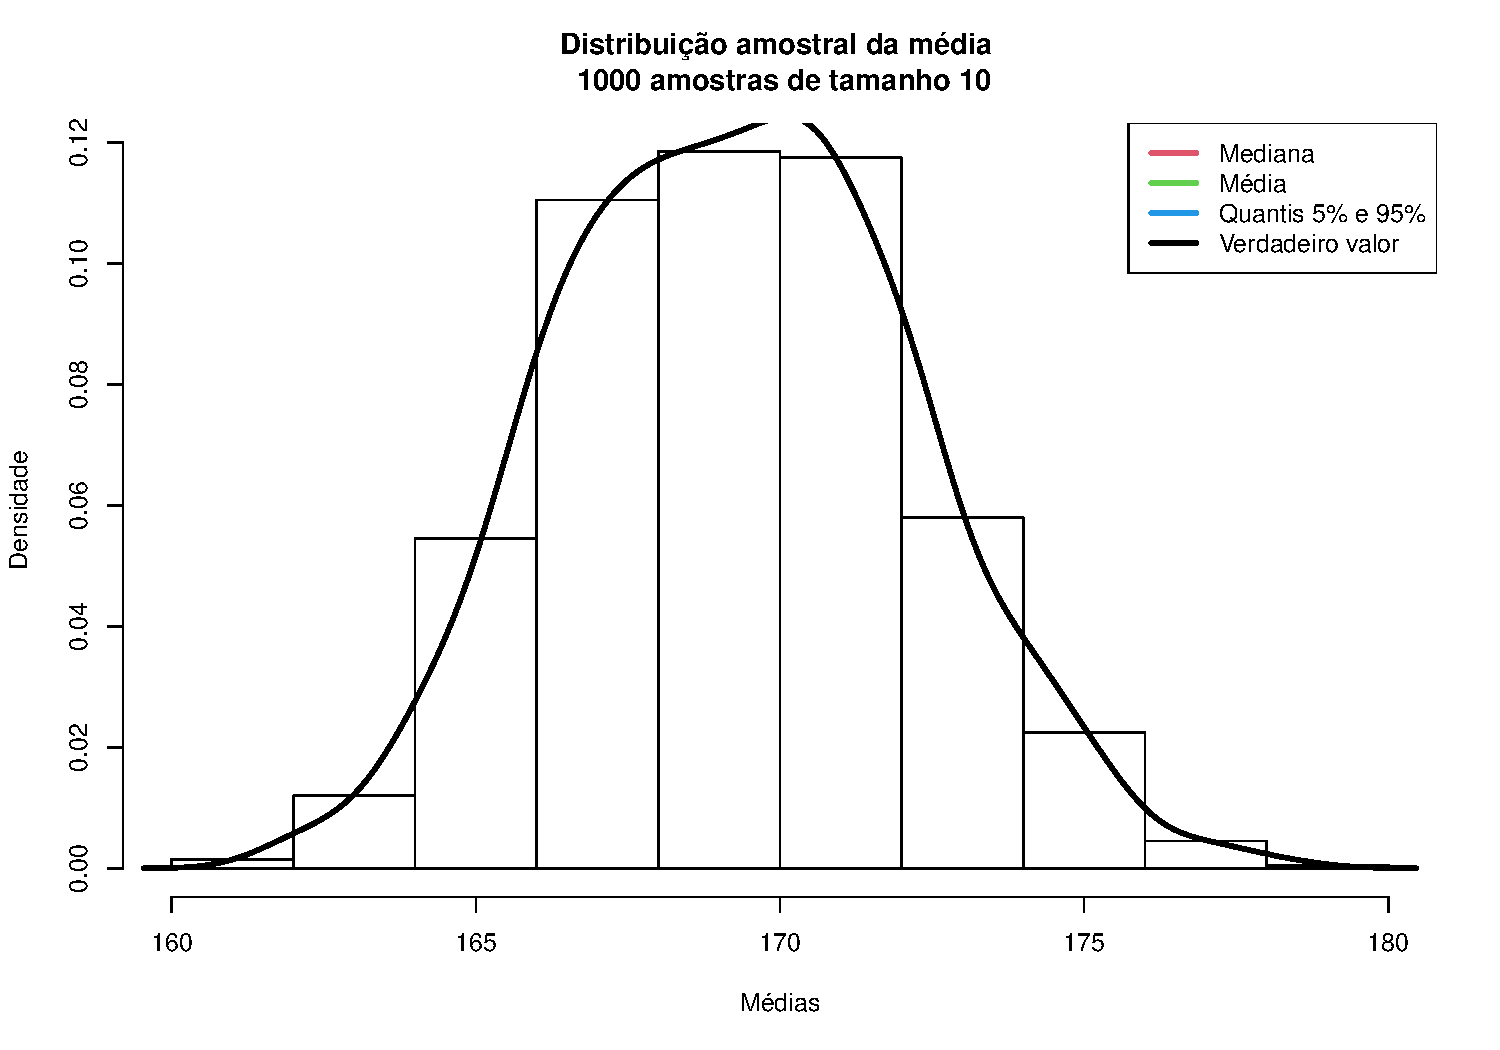
\includegraphics[width=0.7\linewidth]{600-intro-inferencia_files/figure-beamer/unnamed-chunk-1-1} \end{center}
\end{frame}

\begin{frame}{Ilustração computacional}
\protect\hypertarget{ilustrauxe7uxe3o-computacional-3}{}
\begin{center}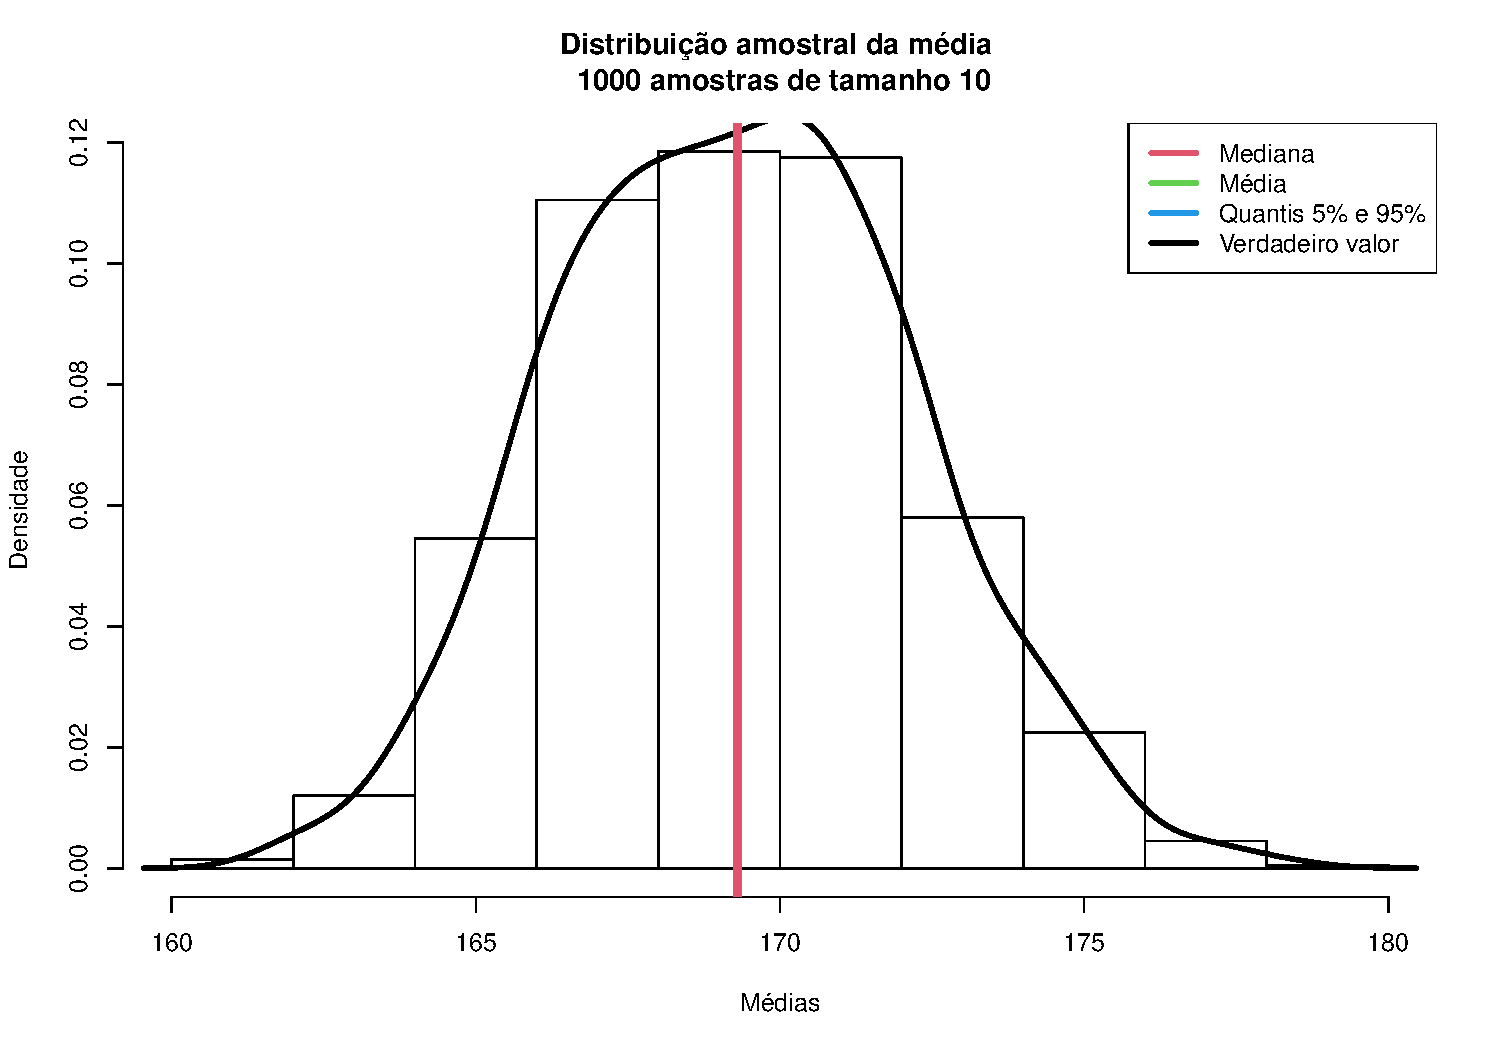
\includegraphics[width=0.7\linewidth]{600-intro-inferencia_files/figure-beamer/unnamed-chunk-2-1} \end{center}
\end{frame}

\begin{frame}{Ilustração computacional}
\protect\hypertarget{ilustrauxe7uxe3o-computacional-4}{}
\begin{center}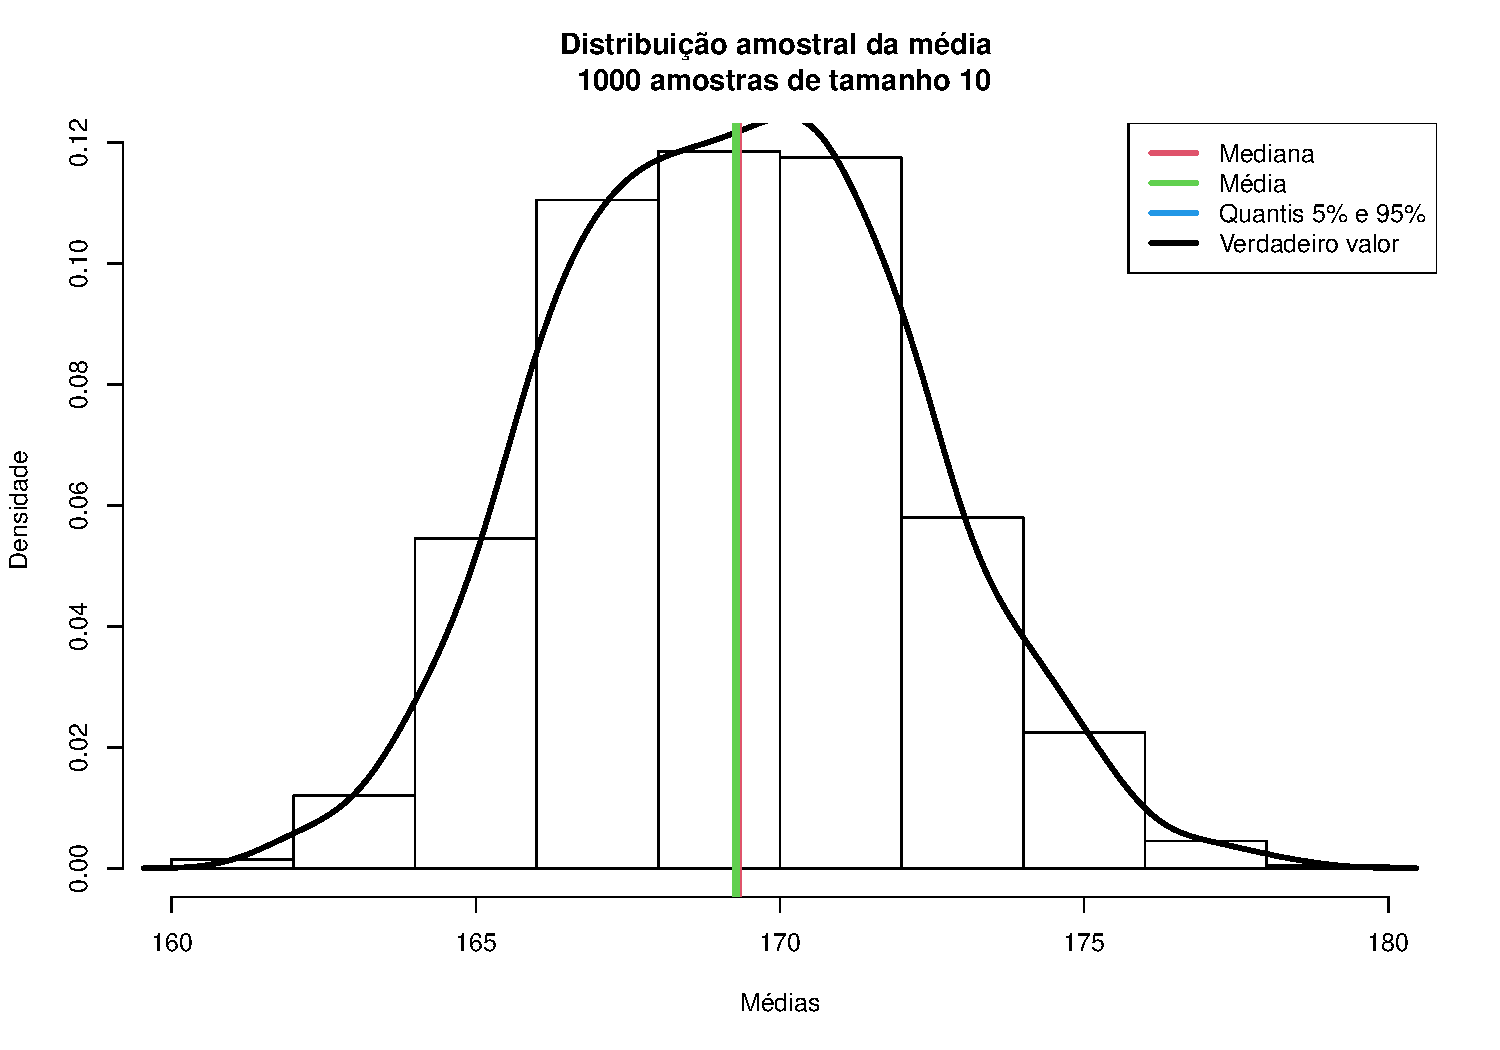
\includegraphics[width=0.7\linewidth]{600-intro-inferencia_files/figure-beamer/unnamed-chunk-3-1} \end{center}
\end{frame}

\begin{frame}{Ilustração computacional}
\protect\hypertarget{ilustrauxe7uxe3o-computacional-5}{}
\begin{center}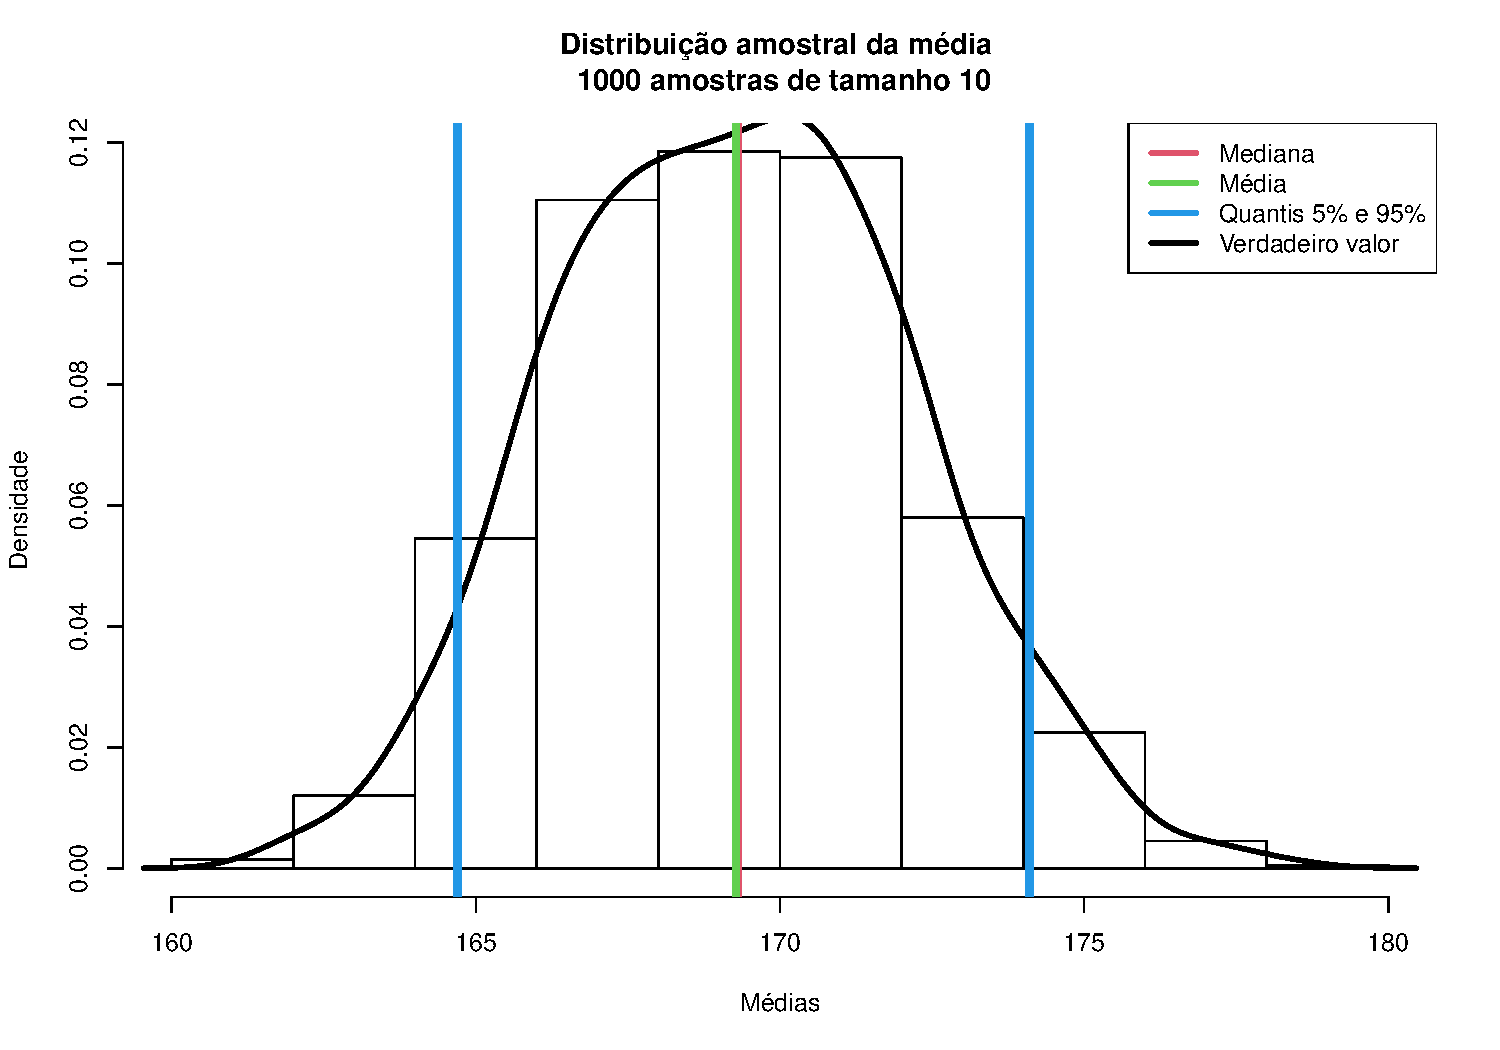
\includegraphics[width=0.7\linewidth]{600-intro-inferencia_files/figure-beamer/unnamed-chunk-4-1} \end{center}
\end{frame}

\begin{frame}{Ilustração computacional}
\protect\hypertarget{ilustrauxe7uxe3o-computacional-6}{}
\begin{center}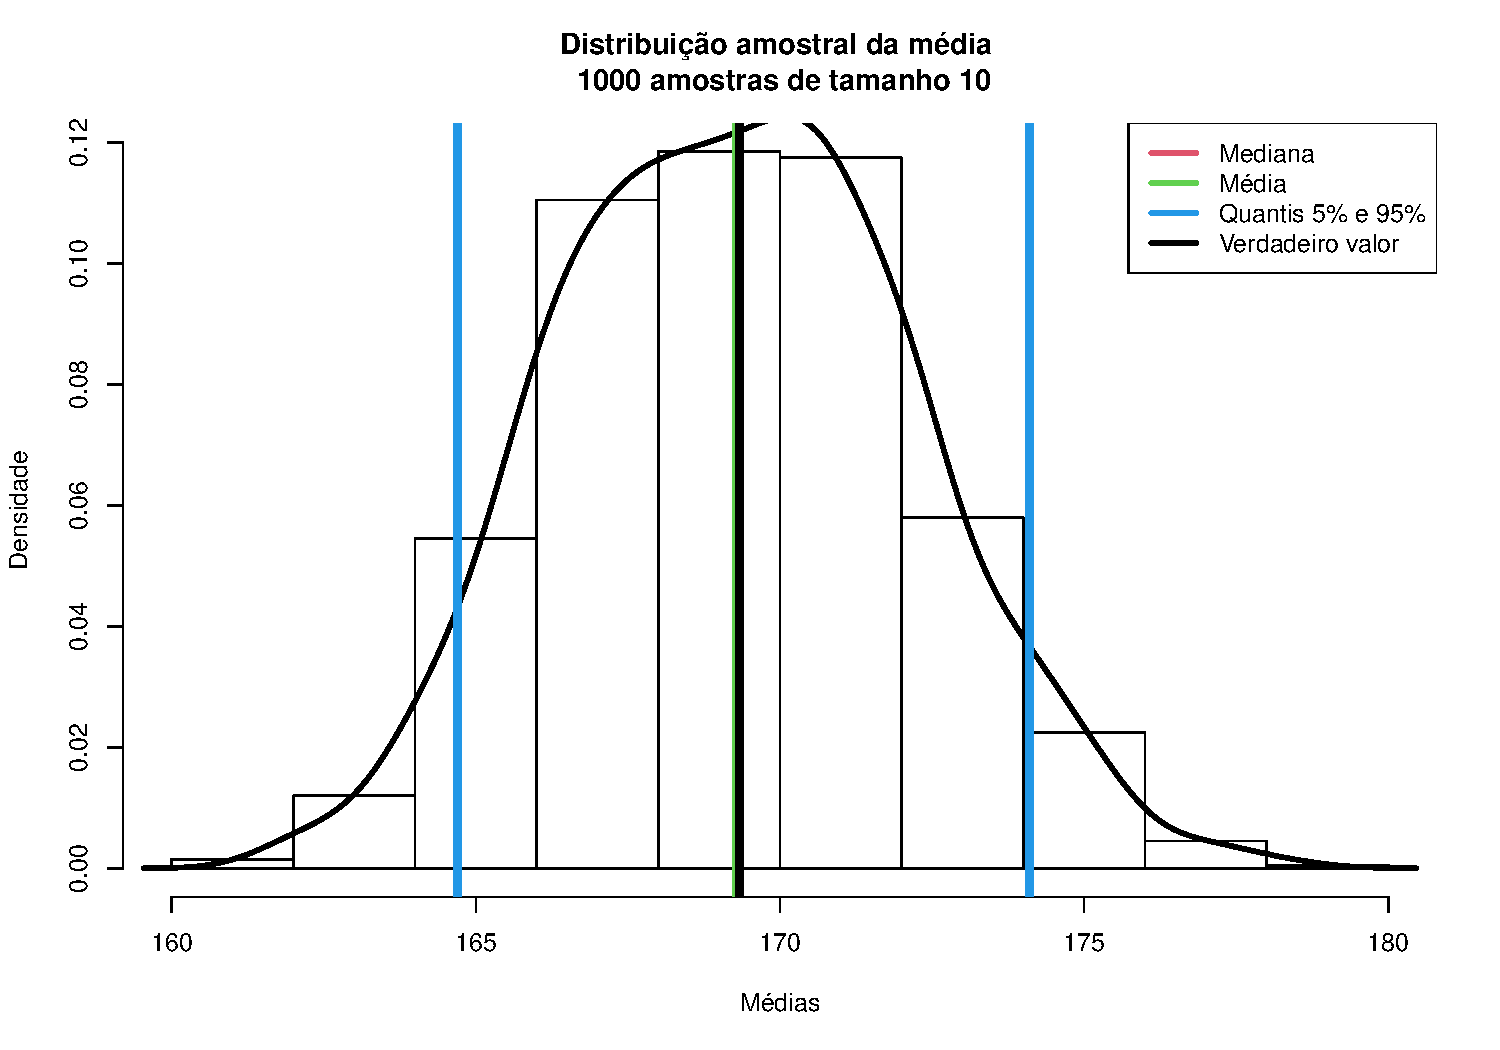
\includegraphics[width=0.7\linewidth]{600-intro-inferencia_files/figure-beamer/unnamed-chunk-5-1} \end{center}
\end{frame}

\begin{frame}{Ilustração computacional}
\protect\hypertarget{ilustrauxe7uxe3o-computacional-7}{}
\begin{itemize}
\tightlist
\item
  Os resultados mostram que não precisamos olhar a população para ter
  uma estimativa satisfatóriamente próxima do verdadeiro valor do
  parâmetro de interesse.
\end{itemize}

\vspace{0.3cm}

\begin{itemize}
\tightlist
\item
  Contudo esta estratégia é inviável na prática, pois necessita de
  várias amostras.
\end{itemize}

\vspace{0.3cm}

\begin{itemize}
\tightlist
\item
  Verificamos que a distribuição amostral é simétrica.
\end{itemize}

\vspace{0.3cm}

\begin{itemize}
\tightlist
\item
  O teorema central do limite garante que esta distribuição é Normal.
\end{itemize}
\end{frame}

\begin{frame}{Ilustração computacional}
\protect\hypertarget{ilustrauxe7uxe3o-computacional-8}{}
\begin{itemize}
\tightlist
\item
  Na prática usamos uma distribuição normal centrada na estimativa de
  uma única amostra.
\end{itemize}

\vspace{0.3cm}

\begin{itemize}
\tightlist
\item
  Com base nesta distribuição amostral estimada, fazemos inferência.
\end{itemize}

\vspace{0.3cm}

\begin{itemize}
\tightlist
\item
  Os quantis desta distribuição garantem a confiança. Neste caso
  tomaremos os quantis 5\% e 95\% da distribuição estimada.
\end{itemize}

\vspace{0.3cm}

\begin{itemize}
\tightlist
\item
  Se replicarmos o procedimento 100 vezes, esperamos que em 10 vezes o
  intervalo dado pelos quantis não contenham o valor do parâmetro.
\end{itemize}
\end{frame}

\begin{frame}{Ilustração computacional}
\protect\hypertarget{ilustrauxe7uxe3o-computacional-9}{}
\begin{center}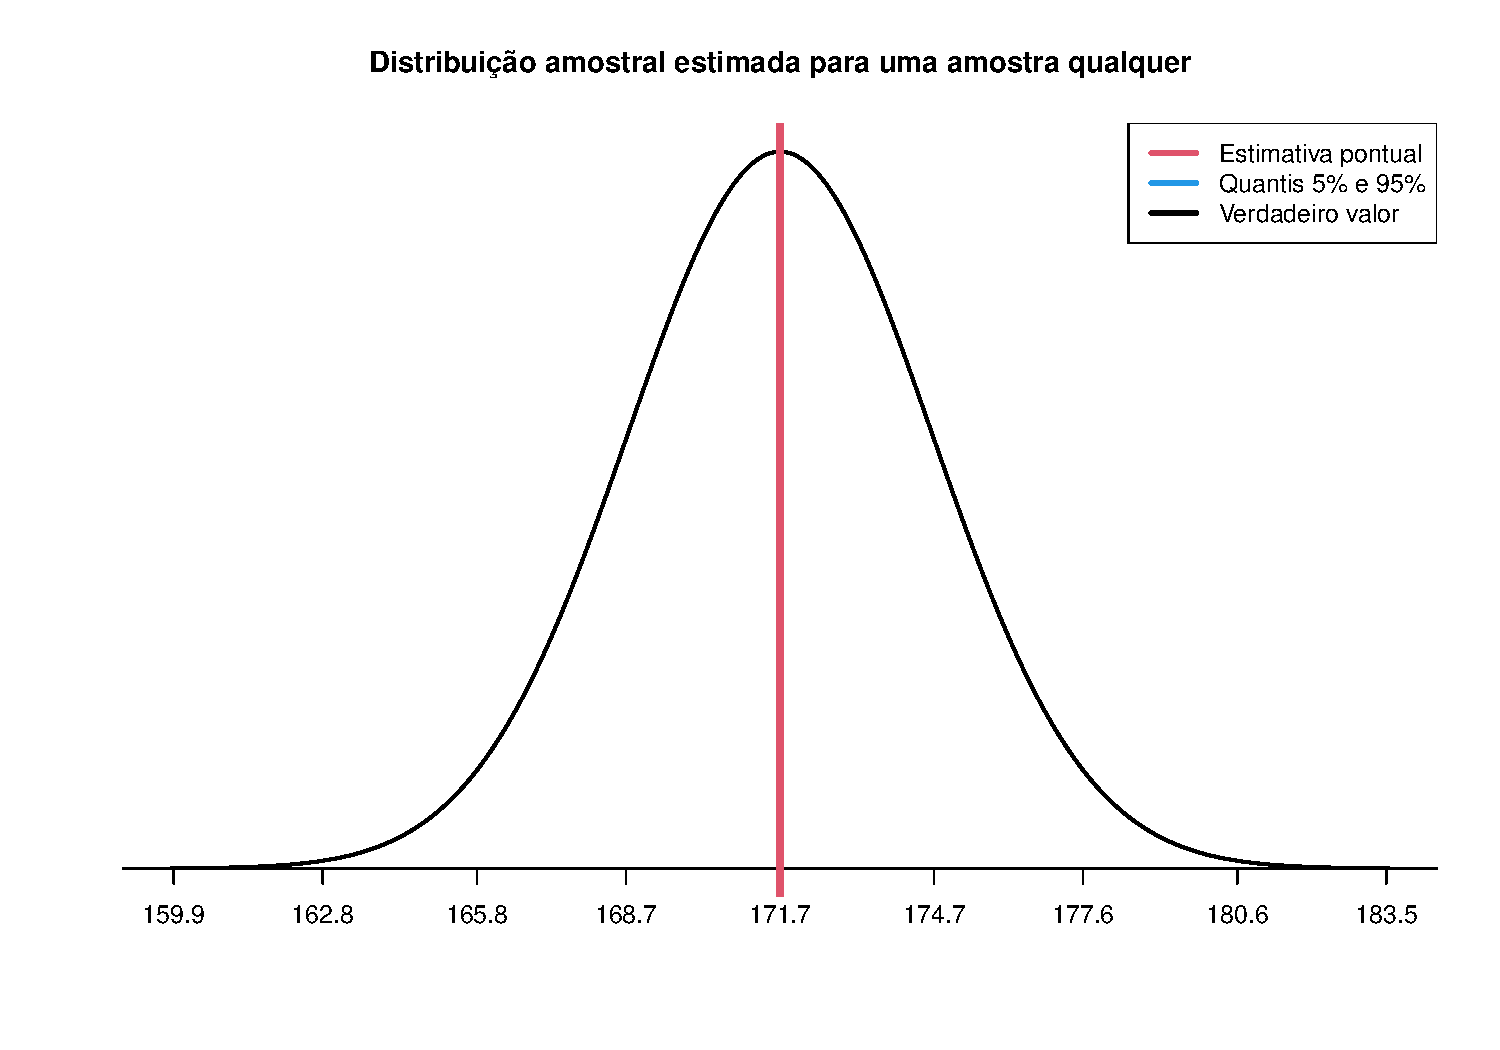
\includegraphics[width=0.7\linewidth]{600-intro-inferencia_files/figure-beamer/unnamed-chunk-6-1} \end{center}
\end{frame}

\begin{frame}{Ilustração computacional}
\protect\hypertarget{ilustrauxe7uxe3o-computacional-10}{}
\begin{center}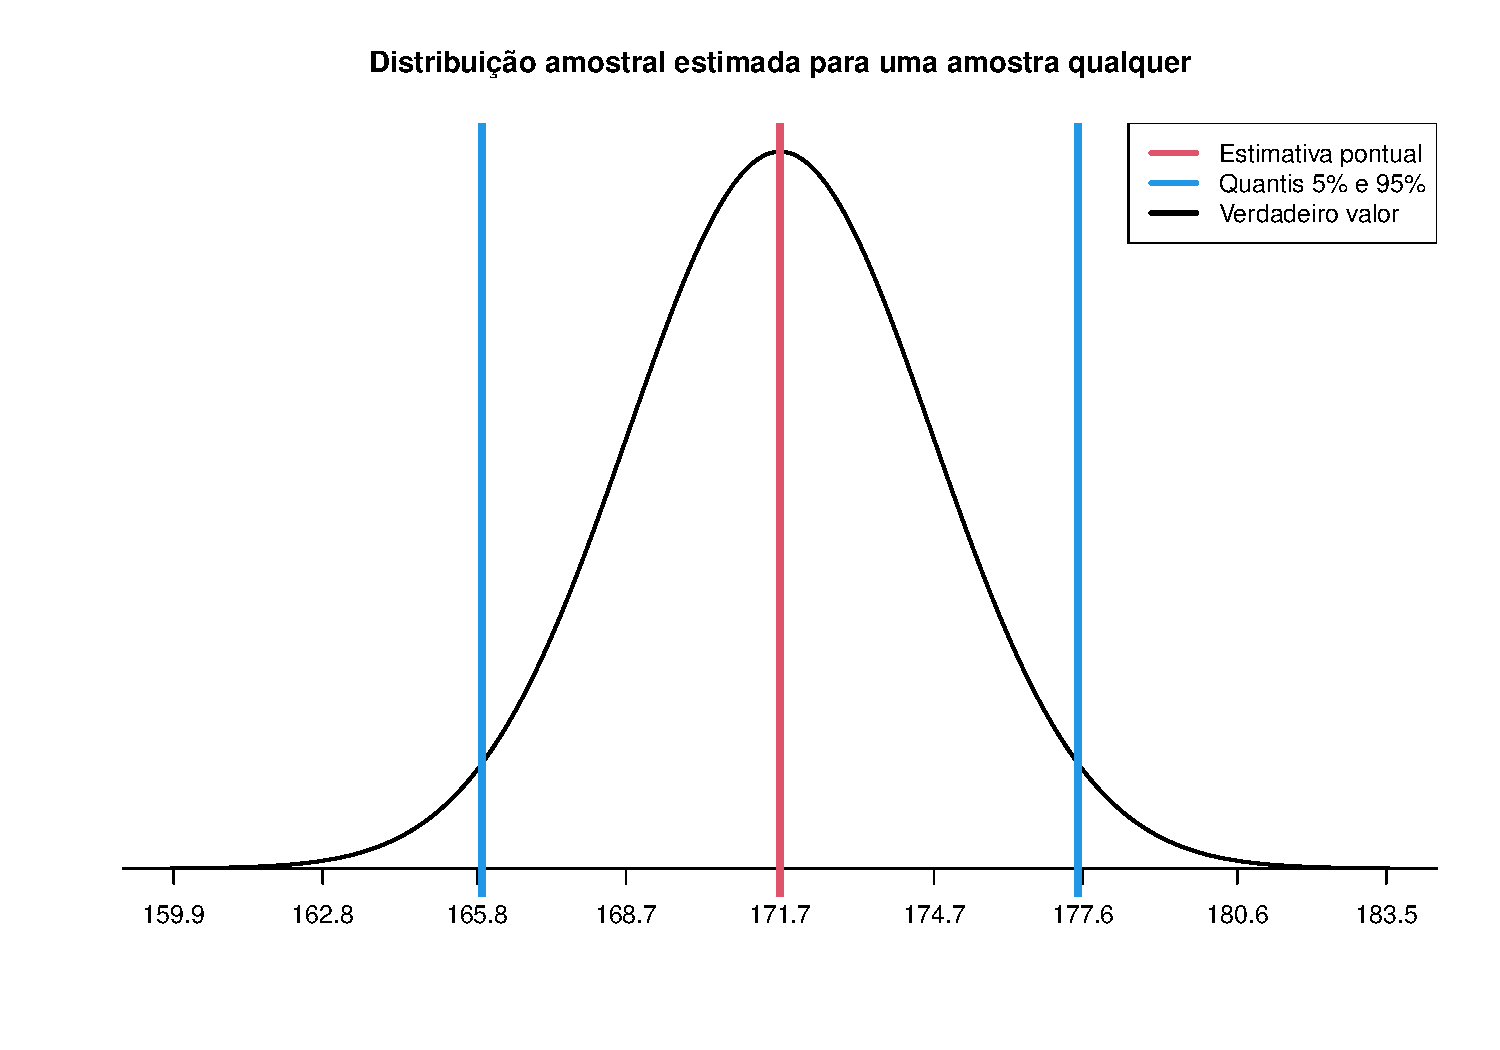
\includegraphics[width=0.7\linewidth]{600-intro-inferencia_files/figure-beamer/unnamed-chunk-7-1} \end{center}
\end{frame}

\begin{frame}{Ilustração computacional}
\protect\hypertarget{ilustrauxe7uxe3o-computacional-11}{}
\begin{center}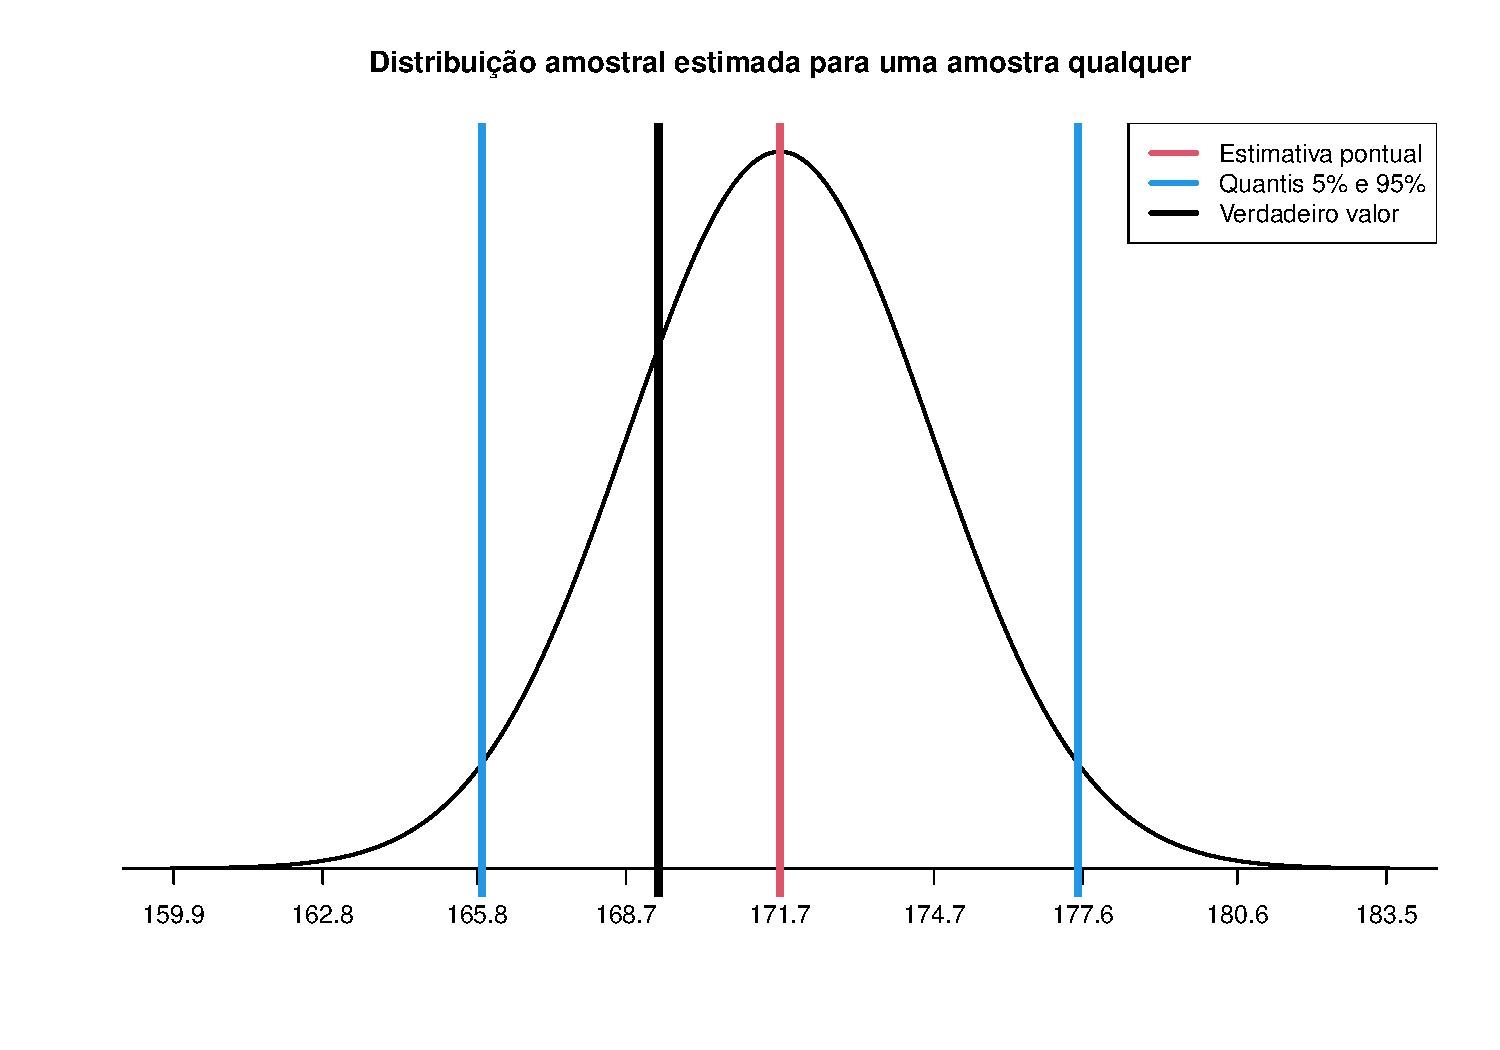
\includegraphics[width=0.7\linewidth]{600-intro-inferencia_files/figure-beamer/unnamed-chunk-8-1} \end{center}
\end{frame}

\begin{frame}{}
\protect\hypertarget{section}{}
\textbf{O que foi visto:}

\begin{itemize}
\tightlist
\item
  Conceitos importantes para inferência estatística.
\item
  Ideia de distribuição amostral.
\item
  Distribuição amostral da média.
\item
  Ilustração computacional.
\end{itemize}
\end{frame}

\end{document}
